\section{Sketch of technique}

We start with robotic system traces from ROS, a published-subscriber architecture for connecting robotic components.  
These traces are called `bags' within the domain of ROS, and contain system messages published on certain data structures (called topics) in chronological order.
Specifically, we will examine trace data from a UAV system used to collect water samples during windy conditions.
Each file might contain 100,000 records, and we have 50-100 bags.

\emph{The ``how" details}

Starting with these bags, we plan to create functions that recognize certain sequences and values of message and record `events' to a new event log.
This event log captures important spatial events during the execution of an automated script, or plan, that lasts about five minutes.
One of the challenges will be creating the functions that recognize these events and determining the correct level of refinement for these events.

At a high level, the stages of model extraction will be:

\begin{itemize}
  \item For each bag file: BAG $\rightarrow$ BAG' $\rightarrow$ BAG'' 

  \item Process the entire collection of BAG'' files to return a spatial model.
\end{itemize}

% This still needs quite a bit of work/editing/thinking...

For each bag file, we will identify basic ``events" that will make up a new BAG' file.  
For this descriptive example, we will only consider the \emph{UP} event, but the technique is the same for the other primitive events.  
First the user will define a granularity of movement significance, such as 0.2 meters, so that any primitive movement which exceeds 0.2 meters will register as an event (or concatenation of events).
We will run checks on each publication of the position data, and if the z-axis position has increased by more than 0.2 meters, we will divide the increase by 0.2, take the floor of the result, call it x, and will write x instances of UP to the BAG' file.  
After we have a BAG' file that logs our primitive events, we will perform a linear scan on this file to check for each spatial property we are interested in.  
For instance, to check for any \emph{BOUNCING} intervals, we will scan the BAG' file for alternating consecutive \emph{UP}s and \emph{DOWN}s. 
These spacial events will be written to a BAG'' file.
The system we will be using publishes a global ``Subject Control State."
So to provide a rough grouping as we scan for each new spatial event, we will write the spatial events to the BAG'' file under the heading of their respective states.
This grouping will hopefully become less coarse throughout the course of implementation.
From the collection of BAG'' files, we will note behaviors which occur more than a predefined number of times as ``common" behaviors to each state for that given task.

\emph{Tool applied to example}

% This will demonstrate our example being parsed to the events "FRONT,FRONT,LEFT,LEFT,LEFT,BACK,BACK,RIGHT,RIGHT,RIGHT" which will then be translated to a "RECTANGLE" event
% How contrived! How trivial! Ah well...
% Because the example doesn't deal with multiple trace bag files, we will explain how a rough model might be extracted from multiple "RECTANGLE" events occuring in state 8...

Applying our tool to the example trace data, assume we set the meaningful primitive events to occur with every change in 0.5 meters. 
As the first BAG' file of primitive events is being created, each row is compared against its immediate successor by examining the difference between the corresponding coordinates.
Examining the first two rows of the example, for the "xpos" change we get $0.0831-0.0519=0.0312$, which is below the threshold of 0.5 meters, so no event in the x-axis will be recorded.  
Similarly, with "ypos", the difference is $0.2014-0.1742=0.0272$, which is also below 0.5, and no event in the y-axis will be recorded.
With "zpos", the difference is $1.7469-1.2231=0.5238$, which is above 0.5 meters, and because it is a positive increase in the z-axis, an event of \emph{UP} will be written to the BAG' file.

Processing all the rows in this way gives a bag file with the series of events: 

\emph{UP,UP,RIGHT,RIGHT,DOWN,DOWN,LEFT,LEFT}

As we process the BAG' file, this series of events will be recognized as a \emph{RECTANGLE} spatial event, which will be written to the BAG'' file.  
Our small example does not deal with multiple bag files, but the idea is that all these bag files will be parsed into separate BAG'' files, and if the above \emph{RECTANGLE} event occured each time in "State 8", then the model will state that in "State 8," the event \emph{RECTANGLE} is probable to occur.

\emph{Techniques/tools/frameworks to be used}

We will write the tool using a scripting language, either Ruby or Python.
We use the idea of confidence thresholds from Daikon to determine when some spatial property is considered "regular" as opposed to "random" across runs. 
For the model extraction component of our tool, we will use segment and interval trees to determine when events occur within states and/or across multiple states.
The spatial events will be based on "templates" which are defined by the occurrence and order of specified primitive events.
We may find it useful to define our primitives in the language of spatial logic found in Peuquet~\etal and spatial constraints found in Bindiganavale~\etal. 

\emph{Description of Solution}
% will add other metrics/clean this up

The precision will be as fine or as coarse as the user defines.
If the user defines events as only registering every 2 meters, a model may be quickly built, but the results may be unhelpful.
If the user defines events as registering every 0.00001 meters, the model will follow the trace data exactly, and the excess information will take a long time to process and will return too many spatial events.
The completeness will also depend on user-defined confidence thresholds.
If some event always occurs or occurs frequently, this property will be captured; if it seldom occurs, it will not be captured.  

\emph{Small Study}

Using a UAV in the NIMBUS lab, we will fly it in certain patterns over multiple runs and see if our tool can derive these spatial properties from the bags.
We will first start with our contrived example of moving in a rectangular motion.  
If this is feasible, we will include multiple events in a single run, such as bouncing followed by rectangular motion.
We will also include periods of erratic motion to see if our tool incorrectly constructs models where none would seem to exist.
If time allows, we may want to consider the partial and total orders of spatial relations, such as "above," "below," "in front of," and "behind" with respect to planes in space.

%\begin{figure}[b]
    %\centering
    %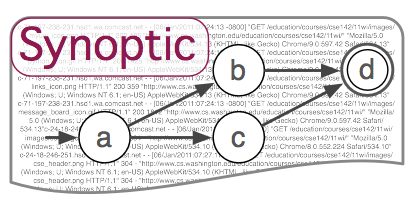
\includegraphics[width=0.4\textwidth]{./figures/TBD.jpg}
    %\caption{Awesome Image}
    %\label{fig:awesome_image}
%\end{figure}
